\section{Motivation}
\label{sec:motivation}

We see two particularily useful scenarios for conflict detection within Floodlight.

\subsection{Debugging Competing Applications}
It is very difficult for an administrator to gain a full understanding of exactly what flow rules get inserted into a switch. 
Applications can be custom made by groups within an enterprise or from some other third party.
With many applications needing to be run on a network, it isn't realistic for an administrator to know every detail of every application that is being run.
There is no guarantee that any two applications, especially when created by third parties, don't logically overwrite each other's rules by accident.
%OpenFlow 1.0 specifies that switches must have support to detect and send an error message when there is an attempt to install a flow rule that has the same or overlapping headers as a rule currently in the flow table.
%This is only done when the \texttt{ADD} request to install the rule has the \texttt{CHECK\_OVERLAP} flag set.
%Otherwise, unless the rules have exactly the same headers, the switch will allow the new rule to be installed "side-by-side" with the old rule.
%When packets come into the switch, they will take the action of the most specific rule that they can match in the flow table.
%If the two rules have exactly the same headers than the new rule will overwrite the old rule.

Flow rules are installed in switches dynamically and are dependent on the traffic flowing through the network.
This can make it extremely difficult for an administrator to investigate undesirable behavior.
The difficulty is exacerbated by the fact that rules are removed from switches due to idle or hard timeouts.
By the time an administrator can inspect the flow table of a switch, its state has most likely already changed.

Thus, it is extremely useful for an admistrator to know when two or more applications are installing rules which logically conflict with each other.
Since all flow rules are installed by the controller, it is the controller that has the ability to build network-wide view of all the flow tables.
This allows the controller to make the difinitive decision to allow, or disallow, a rule to be written to a switch.
Floodlight-CD allows an administrator to debug unintended network behavior due to rule conflicts faster and resolve these conflicts between competing applications.

% Move on the an illustration of a malicious app, talk about the firewall application and how to subvert it, using Floodlight
% in a large network, different groups may want to handle the traffic differently, this would be when they could get the ability to run their own app
% use a campus network for example, each department wants to control its own traffic and have its own application to do it
\begin{figure*}[ht!]
	\begin{center}
		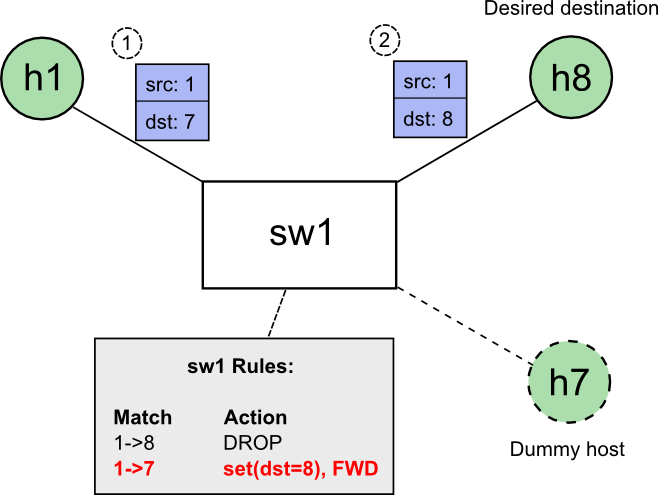
\includegraphics[width=\columnwidth]{figs/singleSwitch_diagram.png}
		\caption{Dynamic flow tunneling using a single switch.}
		\label{fig:dft_single}
	\end{center}
\end{figure*}

\subsection{Malicious Rule Subversion}
While unintentional misconfiguration of applications running on a controller are a definite possibility, we focus on the case where an application author is being intentionally malicious.
% Need more info about dft
As an illustration, we created a simple scenario of dynamic flow tunneling where a malicous application effectively bypasses a firewall rule intended to drop traffic between two hosts.
Figure \ref{fig:dft_single} depicts our example topology.
While this is a somewhat contrived situation (due to the limited number of hosts and simplicity of the applications), the ideas can be extended to larger, real world applications.

The first application acts like a simple ``firewall'' and installs a static rule in every switch to drop any traffic from \texttt{h1} to \texttt{h8} on port \texttt{80}.

\begin{align}
\begin{aligned}
(h1) \rightarrow (h8:80) \Rightarrow Action: drop \nonumber
\end{aligned}
\end{align}

The second application subverts the static rule by dynamically remapping \texttt{h1}'s flow to be redirected from \texttt{h7} towards \texttt{h8}.
This is done by having \texttt{h1} send packets towards a dummy host using port \texttt{80} (the port number is arbitrary, it could be any port as long as the subversive application and the sender are in agreement).

\begin{align}
\begin{aligned}
&(h1) \rightarrow (h7:80) \Rightarrow  \\
    &\qquad Action: set (dst = h8), (port = 80) \nonumber
\end{aligned}
\end{align}

When the switch sees packets destined for the dummy host it, dynamically installs a rule to remap the destinations of those packets from \texttt{h7} to \texttt{h8}.
Since a flow can only match a single rule in a flow table, once the switch remaps the packets' destination, it forwards them on to \texttt{h8} without ever checking them against the firewall's static rule.
%As with network debugging, the controller has a complete view of network and is therefore in a position to arbitrate which rules should be disallowed due to logical conflicts with existing flow rules.


